\section{W�hlen der Client-Distribution}\subsection{Information:}
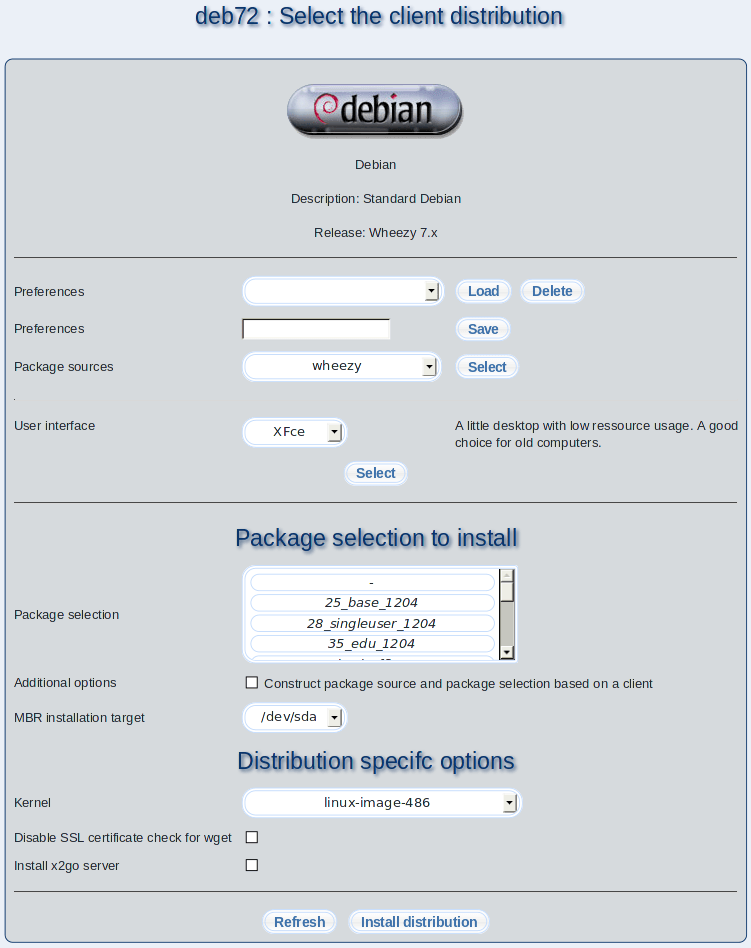
\includegraphics[scale=0.4]{/mdk/doc/manual/screenshots/de/client_distr.png} \\
Eine Distribution ist eine Zusammenstellung von verschiedenen Softwarepaketen, die auf unterschiedlichen Medien (CD, DVD, Internet) vertrieben werden. Es gibt Distributionen, die frei sind und zum kostenlosen Download im Internet angeboten werden. Ein Beispiel daf�r ist  Debian. Unterschiede bei den Distributionen bestehen lediglich in den eingesetzten Installationsprogrammen und der grafischen Aufmachung der Desktops. Die Auswahl einer Distribution ist meist reine Geschmackssache. Um die Unterst�tzung von verschiedenen Client-Distributionen in m23 zu erm�glichen, gibt es nun diesen Auswahl-Dialog.\\
\begin{itemize}
	\item \textbf{Voreinstellungen laden}: W�hlen Sie dazu eine zuvor abgespeicherte Voreinstellung aus der Auswahlliste aus und klicken Sie auf \textit{"Laden"}.\\
	\item \textbf{Voreinstellungen l�schen}: Sie k�nnen eine ausgew�hlte Voreinstellung l�schen, indem Sie auf \textit{"L�schen"} klicken.\\
	\item \textbf{Voreinstellungen speichern}: Die aktuellen Einstellungen k�nnen Sie als Voreinstellung speichern, indem Sie einen Namen eingeben und danach auf \textit{"Speichern"} klicken.\\
	\item \textbf{Paketquellenliste}: Zuerst m�ssen Sie eine Paketquelle ausw�hlen, die Sie unter \textit{Pakete} $\rightarrow$ \textit{Paketquellenliste} erstellt haben. Mit Auswahl der Paketquelle werden gleichzeitig die Distribution, das Release sowie die w�hlbaren Benutzeroberfl�chen festgelegt. Klicken Sie dazu auf \textit{"W�hlen"}. Danach wird das Logo der Distribution zusammen mit einer kurzen Beschreibung oben angezeigt.\\
	\item \textbf{Benutzeroberfl�che}: Abh�ngig von der Paketquelle k�nnen Sie verschiedene Grafische Oberfl�chen ausw�hlen. Alternativ steht \textit{"Textmode"} zur Verf�gung, um einen Server zu installieren, der keinen grafischen Desktop ben�tigt.\\
	\item \textbf{Paketzusammenstellung}: Sie k�nnen hier eine Paketzusammenstellung w�hlen, die zusammen mit dem Betriebssystem installiert wird.\\
	\item \textbf{MBR-Installationsziel}: m23 versucht automatisch die erste Festplatte f�r die Installation des Bootmanagers zu bestimmen. M�chten Sie eine hiervon abweichende Festplatte verwenden, so k�nnen Sie diese hier ausw�hlen. Bedenken Sie, da� dies die Festplatte sein mu�, die vom BIOS zum Booten verwendet wird.\\
	\item \textbf{Distributions-spezifische Einstellungen}: Jede Distribution kann eine Vielzahl von Optionen definieren, die dann zur Installation dieser Distribution genutzt werden.\\
\end{itemize}
Zum Starten der Installation klicken Sie abschlie�end auf \textit{"Distribution installieren"}.\\
\subsection{Hinweis zu Abbilddateien}
W�hlen Sie die Paketquellenliste \textit{"imaging"}, um Abbilddateien zu installieren.\\
Zus�tzlich haben Sie die Wahl, ob Sie den MBR (Master Boot Record) aus einer zuvor erstellten Datei oder den generischen MBR von m23 installieren m�chten, der bootf�hige Partitionen startet. W�hlen Sie hierzu unter \textit{"MBR aus einem Abbild oder generischen MBR installieren"} den Dateinamen oder \textit{"Generischer MBR"}.\\
\subsection{Hinweis:}
Speichern Sie eine Voreinstellung unter dem gleichen Namen ab, unter dem Sie schon Voreinstellungen f�r einen Client gespeichert haben, dann werden die Einstellungen der Distribution hinzugef�gt. Distributions-Einstellungen werden in diesem Fall �berschrieben.\\
